\chapter{Processo de Desenvolvimento do \textit{GAHME Component}}
A engenharia de software baseada em reúso de software é uma estratégia em que o processo de desenvolvimento é orientado para reúso de \textit{softwares} existentes ~\cite{sommerville2011}. Uma abordagem de reúso bastante adota é fazer uso de componentes de \textit{software}que são entidades desenvolvidas com o propósito de serem reutilizadas, incorporando seus comportamentos e funcionalidades no desenvolvimento de novos \textit{softwares}. Essa é uma abordagem é eficaz para esconder a complexidade de um conhecimento especializado que pode ser encapsulado por intermédio do uso dos componentes de software ~\cite{sommerville2011}.

Levando em consideração que os o desenvolvimento de componentes de software para monitoramento de dados de saúde aplicados a jogos eletrônicos (\textit{GAHME Component}), possuem uma complexidade inerente ao domínio em que são aplicados (Saúde). Domínio esse, que necessita de um especialista de domínio (Profissionais de Saúde) para a sua concepção, elaboração e desenvolvimento. Outro grande problema desse contexto é a verificação da eficácia do monitoramento junto aos seres humanos, pois de acordo com as normas regulamentadoras previstas para pesquisa envolvendo seres humanos segundo a Resolução 196/96 ~\cite{conselho2000normas}, qualquer atividade de pesquisa que envolva seres humanos é necessário a submissão a um Comitê de Ética que permita a coleta dos dados. Esse processo leva tempo e pode impactar na produção dos jogos eletrônicos com propósito de monitoramento dos dados de saúde. Logo, se for possível encapsular o conhecimento de domínio em um componente e verificar sua eficácia ~\cite{kato12} junto a seres humanos então os softwares produzidos com o uso destes componentes irão incorporar esse comportamento e não precisarão passar por todo processo de concepção, elaboração e validação da pesquisa em saúde.

Corroborando com esse contexto, Sommerville ~\cite{sommerville2011} cita benefícios do reúso de software que se encaixam perfeitamente neste trabalho:
	\begin{itemize}
		\textbf{Confiança aumentada:} Os softwares reusados, experimentados e testados em sistemas em funcionamento provavelmente são mais confiáveis do que um novo software. Os defeitos podem ser encontrados corrigidos e incorporados novamente nos sistemas melhorando-o continuamente.
		\textbf{Uso Eficaz de especialistas:} Em vez de fazer o levantamento do domínio a ser estudado, os especialistas podem desenvolver \textit{softwares} reusáveis que encapsulam o seu conhecimento;
		\textbf{Desenvolvimento acelerado:} O reúso de um software pode acelerar a produção de um sistema, pois reduz o tempo de desenvolvimento e validação.
	\end{itemize}

A \ac{cbse} surgiu na década de 1990 como uma abordagem para softwares de desenvolvimento de sistemas com base no reúso de componentes de software ~\cite{sommerville2011}. Os componentes são abstrações de nível mais alto do que objetos definidos por usas interfaces. Geralmente eles são maiores que objetos individuais e todos os detalhes de implementação são escondidos de outros componentes ~\cite{sommerville2011}.

Utilizando as técnicas \ac{cbse}, é possível definir, implementar, integrar ou compor componentes independentes, e de fraco acoplamento facilitando o reúso do software ~\cite{bezerra2007}. Essa abordagem facilitou o desenvolvimento de \textit{softwares} cada vez mais complexos, pois por intermédio do reúso e do encapsulamento proporcionado pelos componentes, é possível desenvolve-los e implanta-los com mais agilidade e robustez.  

De acordo com Sommerville ~\cite{sommerville2011}, o desenvolvimento baseado em componentes faz uso de boas práticas de Engenharia de Software, por esse motivo os componentes eles possuem:
	\begin{itemize}
		\item \textbf{Encapsulamento :} como os componentes são especificados por suas interfaces, eles possuem separação entre a definição (interface) e sua implementação. Detalhes de implementação estão encapsulados, podendo ser alterados, modificados sem afetar todo o sistema;
		\item \textbf{Comunicação :} Os componentes comunicam-se por meio de interfaces bem definidas. Se estas interfaces forem mantidas, um componente poderá ser substituído por outro, que forneça melhores resultados;
		\item \textbf{Reúso :} Os componentes devem ser passíveis de composição, todas as interações externas devem ter lugar por meio de interfaces publicamente definidas, permitindo o reúso de software reduzindo o esforço e o tempo gasto de desenvolvimento.		
		\item \textbf{Documentação :} Os componentes devem ser completamente documentados para que os desenvolvedores, possam verificar sua especificação e sua aplicabilidade.
	\end{itemize}

\section{Processo CBSE}
Os processos CBSE são processos de software que oferecem suporte a engenharia de software baseada em componentes. Nesses processos são considerados as possibilidades de reúso e as atividades envolvidas no desenvolvimento e uso de componentes de \textit{software} reusáveis.
Segundo Sommerville ~\cite{sommerville2011}, num nível mais alto existem dois tipos de processo CBSE:
	\begin{enumerate}
		\item \textbf{Desenvolvimento para reúso:} Esse processo está interessado no desenvolvimento de componentes ou serviços que serão reusados em outras aplicações. Esse processo busca generalizar os componentes existentes facilitando o reúso.
		\item \textbf{Desenvolvimento com reúso:} Esse é o processo de desenvolvimento de novas aplicações usando o componentes existentes.
	\end{enumerate}  

O processo básico de um \ac{cbse} (Figura \ref{fig:process-cbse}) com e para reúso apoiam os processos que estão preocupados com a aquisição do componente, gerenciamento de componente e certificação de componente ~\cite{sommerville2011}:

\begin{itemize}
	\item \textbf{Aquisição de componente :} é o processo de aquisição de componentes para reúso ou desenvolvimento em um componente reusável;
	\item \textbf{Certificação de componente :} é o processo de verificação e certificação de que um componente atende a sua certificação.
\end{itemize}

Os componentes podem ser disponibilizados em um repositório, que incluirá as documentações e especificações para o seu uso.

\begin{figure}
 \centering
 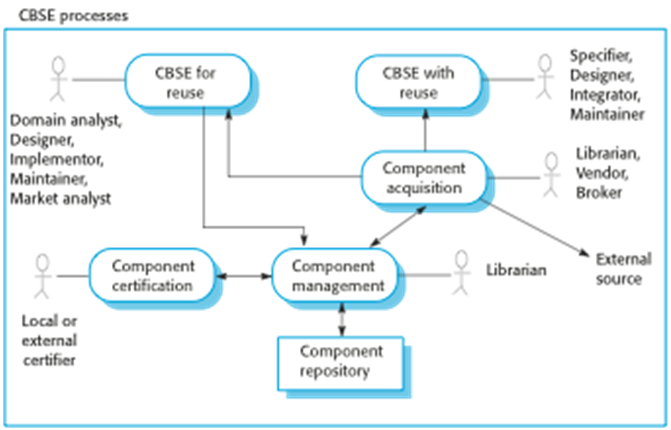
\includegraphics[scale=0.8]{./img/cbse-kot.png}
 % matrixargseg.png: 296x162 pixel, 100dpi, 7.52x4.11 cm, bb=0 0 213 117
 %\caption{Estágio desenvolvimento de jogos ~\cite{fullerton2008game}}
\caption{Processo CBSE}
%  \caption{Estágio desenvolvimento de jogos}
 \label{fig:process-cbse}
\end{figure}

Para a elaboração deste processo foi realizada uma revisão da literatura sobre desenvolvimento de jogos tradicionais (Capítulo \ref{cap:desenvolvimento_jogos}) ~\cite{keith2010agile,moore2011basics,rucker2003,kanode2009} software e das necessidades encontradas no desenvolvimento de jogos voltados para saúde como ~\cite{Suhonen_2010,herber2011,bartolome11,sinclair07,Hardy2011,kato12}. O objetivo desta seção definir um processo de desenvolvimento voltado para reúso que permite desenvolver componentes de \textit{software} a serem integrados em  jogos para entretenimento. Nossa proposta é que esses componentes permitem o monitoramento de dados de saúde de modo não invasivo e integrado a rotina da vida diária.

%Para a elaboração desse processo foram utilizados estudos empíricos através de técnicas de pesquisa qualitativa com o uso de entrevista semi-estruturada \cite{FLI04} e observação participativa em um estudo de caso \cite{Yin05}. O resultado dessas avaliações estã descritos na \secref{section:analise_entrevista_semi_estruturada}. Como resultado dessa análise foram extraídos requisitos (\secref{section:requisitos_entrevista} e \secref{section:requisitos_estudo_caso}) que definiram algumas características e problemas de ambientes distribuídos de desenvolvimento, os quais requerem maior atenção em relação ao desenvolvimento presencial, como: uso de ferramentas colaborativas, meios de comunicação e coordenação das equipes distribuídas. 
%Como procuramos propor um processo completo para ser customizado a toda e qualquer aplicação, é importante que a equipe de desenvolvimento faça uma análise inicial do processo como um todo e de acordo com suas necessidades avalie que atividades e artefatos devem ser instanciados para o projeto.

A modelagem deste processo fez uso da semântica do meta-modelo \ac{spem} na Versão 2.0 \cite{spem08} que permite modelar métodos, atividades de processos de software através da notação gráfica UML. O SPEM 2.0 é usado para definir processos de desenvolvimento de software, sistemas e seus respectivos componentes. O escopo da SPEM se restringe aos elementos necessários para definir qualquer processo de desenvolvimento de software, sem adicionar funcionalidades específicas para domínios particulares (como por exemplo, desenvolvimento de um jogo).

Como pode ser visto na Figura \ref{fig:spem20}, o meta-modelo está estruturado em sete pacotes de meta-modelos. A estrutura divide o modelo em unidades lógicas com responsabilidades bem definidas e cada unidade compartilha informações gerando dependências entre elas sendo capaz de suportar diferentes variedades de clico de vida, como: em cascata, iterativo e incremental, evolucionário e assim por diante.

\begin{figure}
 \centering
 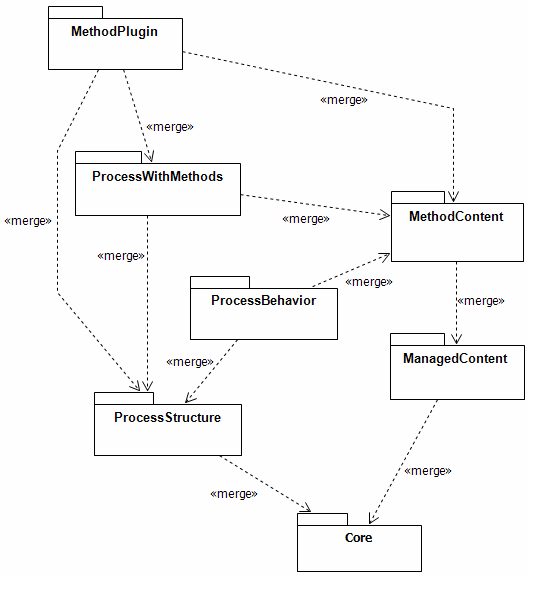
\includegraphics[scale=0.5]{./img/spem20.png}
 % matrixargseg.png: 296x162 pixel, 100dpi, 7.52x4.11 cm, bb=0 0 213 117
 %\caption{Estágio desenvolvimento de jogos ~\cite{fullerton2008game}}
\caption{Estrutura do meta-modelo SPEM 2.0}
%  \caption{Estágio desenvolvimento de jogos}
 \label{fig:spem20}
\end{figure}

Esse processo foi modelado a partir da ferramenta \ac{epf} \cite{epf13}, essa ferramenta é utilizada para autoria de processos através da notação de descrição de processos \ac{spem} \cite{spem08}. A partir dela é possível criar, customizar e publicar os processos de desenvolvimento.

\section{Visão Geral}
O processo proposto, chamado \textbf{GAme Health Monitor Embedded-UFCG Process} (\textit{GAHME Process}), aborda o desenvolvimento componente de software para jogos eletrônicos, com o objetivo monitorar dados de saúde. 

Com o desenvolvimento da proposta, procuramos criar um processo que fosse genérico o suficiente para atender diversos tipos de jogos, mas que contemplasse a capacidade de monitoramento dos dados de modo que o jogo pudesse: capturar dados de saúde, identificar sintomas e validar a proposta do jogo com a ocorrência dos sintomas a serem monitorados. Desta forma, podemos dizer que a principal contribuição deste processo é fornecer um conjunto coerente de atividades e artefatos direcionados para o Desenvolvimento de Jogos Com a Capacidade de Monitorar Dados de Saúde, mas que mantém a generalidade de um processo de desenvolvimento de software podendo ser aplicado no contexto de desenvolvimento de jogos.

\begin{figure}
 \centering
 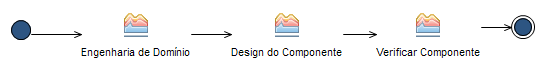
\includegraphics[scale=0.8]{./img/visaogeral.png}
 % matrixargseg.png: 296x162 pixel, 100dpi, 7.52x4.11 cm, bb=0 0 213 117
 %\caption{Estágio desenvolvimento de jogos ~\cite{fullerton2008game}}
\caption{Visão Geral \textit{\ac{gahme} Process}}
%  \caption{Estágio desenvolvimento de jogos}
 \label{fig:visaogeral}
\end{figure}

\begin{figure}
 \centering
 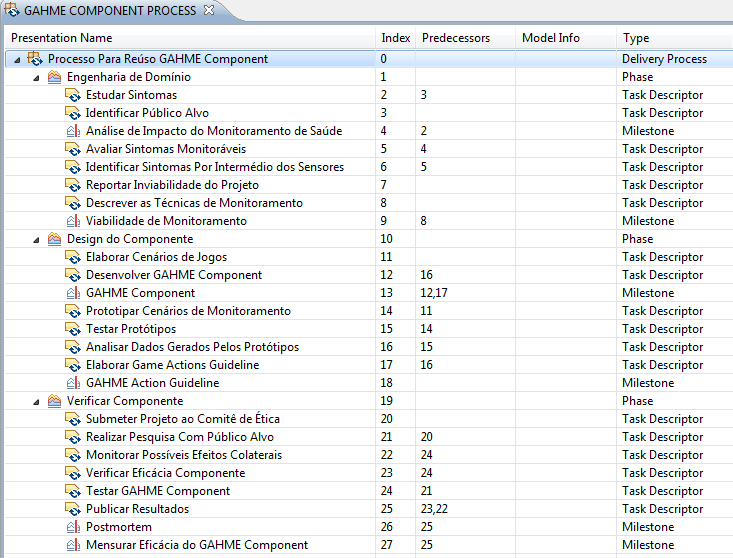
\includegraphics[scale=0.8]{./img/wbs2.png}
 % matrixargseg.png: 296x162 pixel, 100dpi, 7.52x4.11 cm, bb=0 0 213 117
 %\caption{Estágio desenvolvimento de jogos ~\cite{fullerton2008game}}
\caption{Estrutura Analítica do Processo Para Reúso \ac{gahme} Component}
%  \caption{Estágio desenvolvimento de jogos}
 \label{fig:visaogeral}
\end{figure}

\section{Papéis e Responsabilidades}
%Nesta seção serão descritoos os papéis previstos no processo, bem como a descrição de suas principais habilidades e atribuições.

O \textit{GAHME Process} é um processo de jogos eletrônicos que permitem realizar o monitoramento de dados de saúde, a descrição dos papéis presentes no processo se faz importante para um melhor entendimento das atividades realizadas em cada fase do processo.

\subsection{\textit{Game Designer}}\label{subsec:game_designer}
O projeto de um jogo eletrônico requer a contribuição de diversos perfis e habilidades. O \textit{Game Designer} deve trabalhar em colaboração com todos os membros da equipe de desenvolvimento como Engenheiro de Software, \textit{Art Designer} e conhecer também o que o jogador espera encontrar em um jogo ~\cite{schell2008art}. Um bom \textit{Game Designer} está disposto a escutar as diferentes opiniões e sugestões e selecionar aquelas que venham melhorar a experiência do jogo ~\cite{moore2011basics}. Esse papel é responsável pela concepção do jogo, passando por atividades de análise, melhoramento do documento e verificação do resultado final do jogo.

\subsubsection{Habilidades}
Para desempenhar este papel é necessário que o integrante tenha o perfil com as seguintes habilidades:
  \begin{itemize}
	  \item Entender dos anseios e ponto de vista do jogador em relação ao jogo a ser desenvolvido ~\cite{schell2008art};
		\item compreender as ações monitoráveis que o jogador poderá executar definidos no \textit{Game Actions Design} (Seção \ref{subsec:game_actions_guide});
		\item conceber o jogo o que confere a narrativa, regras e objetivos do jogo ~\cite{schell2008art,moore2011basics,bethke2003game}
  \end{itemize}

\subsubsection{Abordagens de Atribuição}
O \textit{Game Designer} deve ter conhecimento sobre as capacidades técnicas da equipe e da \textit{engine} de jogos selecionada para o desenvolvimento do jogo. É essencial que o \textit{Game Designer} conheça sobre as ações que os jogadores precisem desempenhar para serem monitorados. Essa habilidade poderá ser obtida através do \textit{GAHME Actions Guideline}, que conterá a descrição dessas ações.

\subsection{\textit{Game Health Designer}}
O \textit{Game Health Designer} tem um papel bem parecido com o do \textit{Game Designer} (Seção \ref{subsec:game_actions_guide}) contudo deverá trabalhar em colaboração maior com o Profissional de Saúde e do Engenheiro de Software na fase de \textit{Iniciação} onde serão verificadas a viabilidade de um jogo com objetivo de monitoramento de saúde e na elaboração do \textit{Game Actions Design} (\ref{subsec:game_actions_guide}) artefato que fará um mapeamento das ações passíveis de monitoramento e sua relação com os dados de saúde que serão monitorados durante o jogo. Esse último artefato, deverá ser utilizado pelo \textit{Game Designer} para a elaboração do enredo e cenários do jogo.

\subsubsection{Habilidades}
Para desempenhar este papel é necessário que o integrante tenha o perfil com as seguintes habilidades:
  \begin{itemize}
	  \item Compreender as diretrizes médicas (Seção \ref{subsec:diretrizes_medicas}) e conseguir extrair sintomas monitoráveis com o auxílio do Profissional de Saúde;
		\item analisar as possibilidades de monitoramento por intermédio dos sensores disponíveis e com o auxílio do Engenheiro de Software que irá verificar a viabilidade do monitoramento;
		\item verificar a viabilidade do monitoramento dos dados de saúde por intermédio de um jogo eletrônico;
		\item conceber um artefato de \textit{Game Actions Design} que auxilie na concepção do jogo por parte do \textit{Game Design}.
  \end{itemize}

\subsubsection{Abordagens de Atribuição}
O \textit{Game Health Designer} deve ter conhecimento tanto da área de saúde quanto das tecnologias utilizadas no desenvolvimento dos jogos.


% In the last few months of production, the focus shifts from producing new code and features to making certain that what has already been built functions as expected and that the levels and artwork are complete and polished. The team shrinks down in size because the majority of production artists and outside talent such as sound designers and writers are no longer needed ~\cite{fullerton2008game}.


\section{Fase: Engenharia de Domínio}
O objetivo da iteração de Engenharia de Domínio é identificar o impacto que o jogo para o monitoramento de dados de saúde trará e avaliar se será possível desenvolver esse jogo com a tecnologia atual.

\begin{figure}
 \centering
 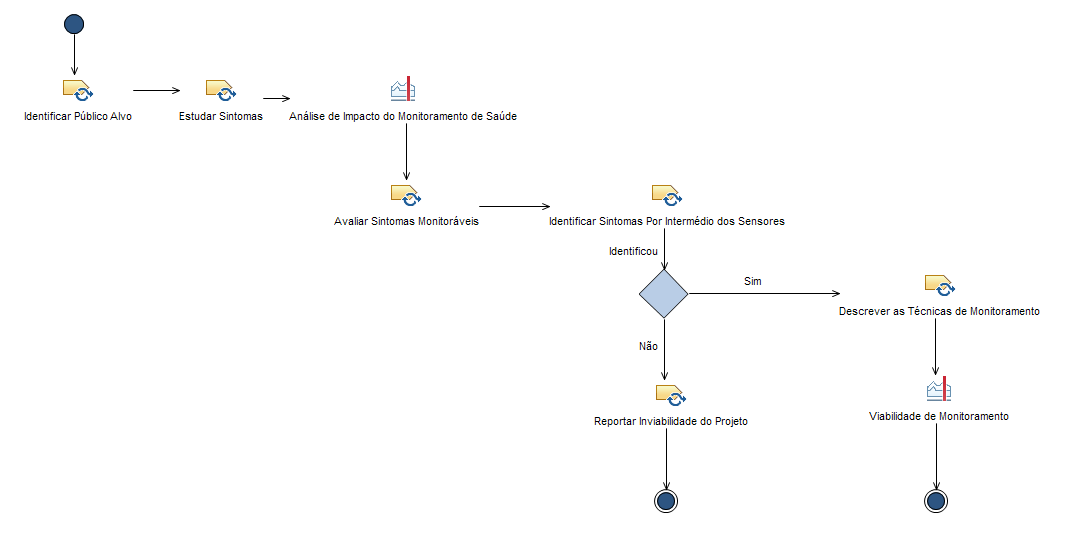
\includegraphics[scale=0.55]{./img/engenhariadominio.png}
 % matrixargseg.png: 296x162 pixel, 100dpi, 7.52x4.11 cm, bb=0 0 213 117
 %\caption{Estágio desenvolvimento de jogos ~\cite{fullerton2008game}}
\caption{Fase: Engenharia de Domínio do \textit{GAHME Process} Orientado à Reúso}
%  \caption{Estágio desenvolvimento de jogos}
 \label{fig:iniciacao}
\end{figure}

\subsection{Atividade: Identificar Público Alvo}
Primeiramente o \textit{Game Health Designer} deverá encontrar qual é o perfil do jogador, essa é uma questão importante, pois irá definir o público alvo do jogo. Se será destinado a um público que já possui o hábito de jogar jogos eletrônicos ou a um público com um nível de habilidade menor. Se haverá sistema de balanceamento de dificuldades tentando atender os dois públicos ~\cite{brathwaite2009challenges}. É necessário também avaliar a faixa etária a que se destina o jogo, pois jogos desenvolvidos para um público infantil tem um perfil bastante diferente dos voltados para adultos ~\cite{brathwaite2009challenges}, e isso irá impactar diretamente na elaboração do \texit{Game Design} do projeto, pois deve-ser levado em consideração que as crianças preferem ambientes mais lúdicos ~\cite{yannakakis06}, e pessoas idosas devem e precisam de jogos não os ponha em situação de risco de saúde como quedas ou fadiga muscular ~\cite{brox11,arntzen2011}.
Para a execução desta atividade o \textit{Game Health Designer} deverá fazer uso do Documento de Diretrizes Médicas (Seção \ref{subsec:diretrizes_medicas}) para identificar a necessidade de monitoramento dos sintomas, juntamente com o Profissional de Saúde, deverão selecionar sintomas que identifique problemas de saúde e que sejam mensuráveis por intermédio de sensores. Durante a execução desta atividade também deve ser coletado as informações a respeito da importância, impactos e benefícios ao tratamento de saúde o público alvo terá ao ter esses sintomas monitorados.

\subsubsection{Papéis Responsáveis}
\begin{itemize}
	\item \textit{Game Health Designer};
	\item Profissional de Saúde.
\end{itemize}

\subsubsection{Passos para Execução da Atividade}
\begin{itemize}
	\item Avaliar faixa etária;
	\item avaliar necessidade de monitoramento;
	\item avaliar sintomas a ser monitorados.
\end{itemize}

\subsubsection{Artefatos de Entrada}
\begin{itemize}
	\item Diretrizes Médicas.
\end{itemize}

\subsubsection{Artefatos de Saída}
\begin{itemize}
	\item Documento de Análise de Impacto.
\end{itemize}


\subsection{Atividade: Estudar Sintomas}
O objetivo principal dessa atividade é identificar sintomas passíveis de monitoramento por meio das Diretrizes Médicas que servirão de base científica para a execução desta atividade. Nessa atividade não deve ser levada em consideração a existência ou especificações técnicas dos sensores, isso será realizado posteriormente na atividade de Viabilidade do Monitoramento. O estudo dos sintomas será baseado nas diretrizes médicas, por meio destas o \textit{Game Health Design} irá mapear os sintomas e valores que identifiquem a sua ocorrência.
%No artefato de saída dessa atividade (Documento de Sintomas Passíveis de Monitoramento) deverão estar presentes os sintomas e possíveis valores para cada sintoma coletado.

\subsubsection{Papéis Responsáveis}
\begin{itemize}
	\item \textit{Game Health Designer};
	\item Profissional de Saúde.
\end{itemize}

\subsubsection{Passos para Execução da Atividade}
\begin{itemize}
	\item Estudar sintomas monitoráveis;
	\item Descrever sintomas passíveis de monitoramento;
	%\item Especificar valores que identifiquem os sintomas;	
\end{itemize}

\subsubsection{Artefatos de Entrada}
\begin{itemize}
	\item Diretrizes Médicas.
\end{itemize}

\subsubsection{Artefatos de Saída}
\begin{itemize}
	\item Documento de Sintomas Passíveis de Monitoramento.
\end{itemize}


\subsection{Atividade: Pesquisar População Beneficiada}
\subsubsection{Papéis Responsáveis}
\begin{itemize}
	\item \textit{Game Health Designer};
	\item Profissional de Saúde.
\end{itemize}

\subsubsection{Passos para Execução da Atividade}
\begin{itemize}
	\item Identificar público alvo
	\item 
\end{itemize}

\subsubsection{Artefatos de Entrada}
\begin{itemize}
	\item Diretrizes Médicas.
\end{itemize}

\subsubsection{Artefatos de Saída}
\begin{itemize}
	\item Documento de Sintomas Passíveis de Monitoramento.
\end{itemize}

\section{Fase: Verificar Componente}
Nos últimos anos houve um crescimento de jogos voltados para saúde, contudo muito desses jogos não foram validados efetivamente ou foi realizado um estudo para verificar os seus resultados ~\cite{kato12}. Os estudos realizados por muitos desses jogos, foram mal projetados e suas conclusões não podem se consideradas validas ou eficazes. Por esse motivo Kato ~\cite{kato12}, sugeriu diretrizes para a realização de estudos de eficácia para ser aplicados em jogos para saúde. 
Como a iteração de "Verificação" é responsável por avaliar a eficácia do monitoramento dos dados de saúde a partir do jogo desenvolvido, as sugestões definidas por Kato ~\cite{kato12} estarão presentes no decorrer da iteração.

Para Kato ~\cite{kato12}, os jogos para saúde precisam passar por pesquisa entre seres humanos e testado com grupo de controle para verificar sua eficácia. Deste modo, os jogos para monitoramento de saúde devem ser submetidos a testes com usuários para verificar se os sinais dos jogadores estão sendo capturados corretamente durante a execução de uma partida. Com o sucesso da execução desta etapa pode ser afirmado que foi desenvolvido um jogo com o propósito de monitoramento de dados de saúde.

\begin{figure}
 \centering
 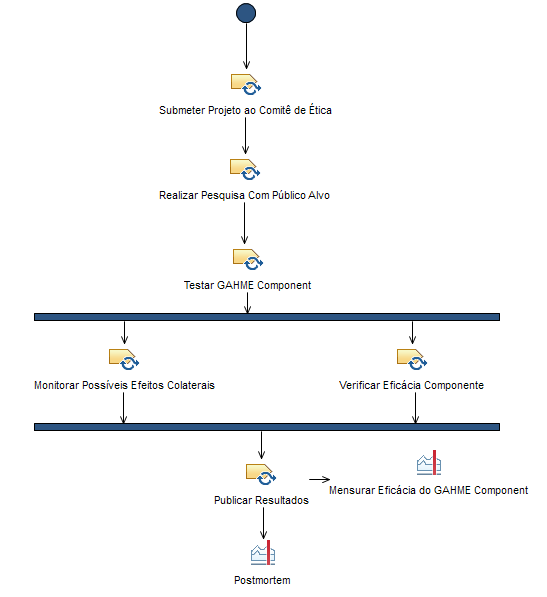
\includegraphics[scale=0.55]{./img/verificar-componente.png}
 % matrixargseg.png: 296x162 pixel, 100dpi, 7.52x4.11 cm, bb=0 0 213 117
 %\caption{Estágio desenvolvimento de jogos ~\cite{fullerton2008game}}
\caption{Iteração: Verificação do \textit{GAHME Process}}
%  \caption{Estágio desenvolvimento de jogos}
 \label{fig:verificação}
\end{figure}

\subsection{Submeter Projeto ao Comitê de Ética}
O objetivo dessa atividade é submeter o jogo às normas regulamentadoras previstas para a pesquisa envolvendo seres humanos segundo a Resolução 196/96 ~\cite{conselho2000normas}. Segundo o Conselho Nacional de Saúde ~\cite{conep2002}, o \ac{cep} é um colegiado interdisciplinar e independente,  que deve existir nas instituições que realizam pesquisas envolvendo seres humanos no Brasil, criado para defender os interesses dos sujeitos da pesquisa em sua integridade e dignidade e para contribuir no desenvolvimento da pesquisa dentro de padrões éticos (Normas e Diretrizes Regulamentadoras da Pesquisa Envolvendo Seres Humanos - Res. CNS 196/96 ~\cite{conselho2000normas}). 

O \ac{cep} é responsável pela avaliação e acompanhamento dos aspectos éticos de todas as pesquisas envolvendo seres humanos. Este papel está bem estabelecido nas diversas diretrizes éticas internacionais (Declaração de Helsinque, Diretrizes Internacionais para as Pesquisas Biomédicas envolvendo Seres Humanos – CIOMS) e Brasileiras (Res. CNS 196/96 e complementares~\cite{conselho2000normas}), diretrizes estas que ressaltam a necessidade de revisão ética e científica das pesquisas envolvendo seres humanos, visando a salvaguardar a dignidade, os direitos, a segurança e o bem-estar do sujeito da pesquisa ~\cite{conep2002}.

Nessa atividade deve ser elaborado um Protocolo de Pesquisa, contemplando a descrição da pesquisa, estabelecer critérios de inclusão e exclusão dos sujeitos da pesquisa, a qualificação dos pesquisadores e todas instâncias responsáveis pelo projeto. Devem fazer presentes no projeto Instituições de pesquisa, legitimamente constituída e habilitada que permita realizar as investigações científicas. 

Os pesquisadores, deverão elencar os riscos da pesquisa, principalmente danos físicos, psíquicos, moral, intelectual, cultural do ser humano em qualquer fase de uma pesquisa dela decorrente ~\cite{conselho2000normas}. Sendo necessária a anuência do sujeito da pesquisa ou de um representante por intermédio do Consentimento livre e esclarecido, onde será explicado a natureza da pesquisa, seus objetivos, métodos, benefícios previstos, potenciais riscos e o incômodo que esta possa acarretar, formulada em um termo de consentimento, autorizando sua participação voluntária na pesquisa ~\cite{conselho2000normas}. Caso o sujeito da pesquisa se enquadre nos critérios estabelecidos para interromper a pesquisa, essa deverá ser finalizada assegurando a integridade do mesmo.

Atualmente no Brasil para poder testar o jogo com monitoramento de dados de saúde junto a pacientes e testar de fato a eficácia do jogo é necessário passar por esse processo e obter a aprovação de um \ac{cep}. Esse é um processo demorado e pode impactar bastante a entrega final.


\subsection{Realizar Pesquisa com Público Alvo}
Durante a pesquisa com o público alvo, o pesquisador deverá ter a preocupação com a integridade do sujeito da pesquisa.
Para isso deverá obedecer o que ficou definido nos "Critérios Para Interromper a Pesquisa" no projeto aprovado pelo \ac{cep}. Segundo a Resolução 196/96 ~\cite{conselho2000normas} caso o pesquisador identifique risco ou dano à saúde do sujeito participante da pesquisa e que não esteja presente no termo de consentimento, o pesquisador é obrigado a suspender a pesquisa. Do mesmo modo, caso haja um método mais seguro para realizar a pesquisa, o projeto deverá ser suspenso, oferecendo a todos os sujeitos os benefícios do melhor regime ~\cite{conselho2000normas}.

Na seção de Riscos e Benefícios da Resolução 196/96 ~\cite{conselho2000normas}, fica fadado ao pesquisador,patrocinador e a instituição devem assumir a responsabilidade de dar assistência integral às complicações e danos decorrentes dos riscos previstos. Os sujeitos da pesquisa que vierem a sofrer qualquer tipo de dano previsto ou não no termo de consentimento e resultante de sua participação, além do direito à assistência integral, têm direito à indenização. Jamais poderá ser exigido do sujeito da pesquisa, sob qualquer argumento, renúncia ao direito à indenização por dano. O formulário do consentimento livre e esclarecido não deve conter nenhuma ressalva que afaste essa responsabilidade ou que implique ao sujeito da pesquisa abrir mão de seus direitos legais, incluindo o direito de procurar obter indenização por danos eventuais.

\subsection{Monitorar Possíveis Efeitos Colaterais}
Durante a execução da pesquisa possíveis efeitos colaterais devem ser monitorados como: risco de queda, fadiga, tendinite. 
s avaliações de jogos para a saúde devem tentar controlar o uso de seu jogo para efeitos colaterais negativos. possível negativo efeitos colaterais dos jogos, embora rara, pode incluir convulsões, devido à fotossensibilidade e tendinites.

\subsection{Verificar Eficácia do Jogo}
A eficácia do jogo será verificada através de um estudo analítico de caso-controle ~\cite{menezes2001epidemiologia}, dentro de um ambiente aprovado pelo \ac{cep} que permitirá recrutar sujeitos de pesquisa. Uns sujeitos deverão apresentar os sintomas a serem monitorados e outros não terão tais sintomas. Os dados serão coletados e ao final deverá ser verificado se os sintomas foram corretamente identificados.

Kato ~\cite{kato12}, defende que para essa verificação é necessário obter um número adequado de participantes para conseguir avaliar o impacto do jogo. Contudo, determinados sintomas possuem poucos sujeitos de pesquisa disponíveis reduzindo a abrangência da pesquisa.

Em uma revisão sistemática sobre a eficácia dos jogos existes e que promovem a atividade física para adolescentes ~\cite{foley-active-game2010}, segundo a revisão a abordagem de jogos se mostrou eficaz ao motivar a execução de atividade física dos usuários. Os jogos estudaram envolveram tanto os membros superiores quanto inferiores do corpo melhorando a atividade de forma prazerosa e com qualidade inclusive em grupos de deficiência e de alto risco.

%Verificar essa referencia ~\cite{Primack2012630}

\subsection{Publicar Resultados}
\section{Artefatos}

Os documentos para o desenvolvimento de jogos tem dois propósitos principais: histórico do projeto e comunicação ~\cite{schell2008art}. O desenvolvimento de um jogo requer a tomada de decisões a todo o momento, que definem o funcionamento do jogo. Contudo, existe uma grande probabilidade de que os envolvidos do projeto não se recordem dos motivos que as decisões forma tomadas. Se a equipe de desenvolvimento tiver o hábito de armazenar todas as tomadas de decisões e documentá-las nos artefatos utilizados no desenvolvimento do software então não será necessário rediscutir as decisões já tomadas ~\cite{schell2008art}.
Os artefatos de software são importantes para comunicar sobre as decisões tomadas durante a concepção do projeto a todos os participantes do mesmo. É importante salientar que em um processo de software os artefatos servem como documentos de entrada e saída da execução de atividades dentro do próprio processo ~\cite{sommerville2011}.

\subsection{Diretrizes Médicas}\label{subsec:diretrizes_medicas}
O principal propósito da atividade médica é o cuidado do paciente, e isso traz enormes desafios de forma coletiva ou individual. Com o intuito de auxiliar na tomada de decisões, a comunidade médica mundial tem elaborado e divulgado um extenso número de informações ~\cite{nhs2013,neozeland-guide-2013}, muito mais acessíveis do que era no passado, redefinindo o universo do conhecimento médico, tornando-o livre e acessível para críticas e demais propósitos científicos ~\cite{proj-diretriz2013}.

Neste contexto, a Associação Médica Brasileira e o Conselho Federal de Medicina, também com o objetivo de auxiliar na decisão médica e, consequentemente, otimizar o cuidado aos pacientes, desencadearam um processo junto às Sociedades de Especialidade para a elaboração de Diretrizes Médicas baseadas nas evidências científicas disponíveis na atualidade ~\cite{proj-diretriz2013}.
Nesse processo, formou-se por uma Comissão Técnica responsável em construir as bases de sustentação das recomendações de conduta médica, utilizando os meios da ciência atual, de forma crítica e desprovida de interesse se não aquele que resulte na melhoria do tratamento do médico com o paciente. 

Partindo do princípio que o conhecimento médico atual está presente nas diretrizes médicas e que através do seu conteúdo é possível 	extrair informações que permitam identificar e avaliar a presença e evolução de sintomas de doenças, esse artefato será de extrema importância para o desenvolvimento de um jogo eletrônico com o objetivo de realizar o monitoramento de dados de saúde.
%Nas diretrizes médicas estão descritos mecanismos de diagnósticos, prognóstico, tratamento, dosagem medicamentosa, riscos e benefícios. Além de definir questões mais relacionadas à prática clínica e descrevendo as possíveis opções para a tomada de decisão sobre o tratamento da doença .a ser monitorada como por exemplo a Doença de Parkinson que servirá como estudo de caso do presente trabalho ~\cite{protpar010}.
%evidências através dos dados sobre a doença bem como mecanismos de diagnósticos, prognóstico, tratamento, dosagem medicamentosa, riscos e benefícios. Além de definir questões mais relacionadas à prática clínica e descrevendo as possíveis opções para a tomada de decisão sobre o tratamento da doença .a ser monitorada como por exemplo a Doença de Parkinson que servirá como estudo de caso do presente trabalho ~\cite{protpar010}.
\subsubsection{Propósito}
As diretrizes médicas permitem identificar sintomas passíveis de monitoramento, bem como parâmetros  relevantes a esses sintomas. As diretrizes médicas são documentos produzidos por sólidas bases científicas, sendo escrita pela própria comunidade médica que determina seus representantes. Por esse motivo, esse documento passa por rigorosas revisões e em constantes atualizações, sendo uma das principais referências para os profissionais da saúde. Para o \textit{GAHME Process} este artefato servirá de base científica para fundamentar quais sintomas serão monitorados e de que forma serão avaliados.


%\subsection{Estudos Epidemiológicos}\label{subsec:estudos_epidemiologicos}
%A Epidemiologia é a ciência que estuda ocorrência de doenças em populações humanas e seus fatores determinantes das doenças ou condições relacionadas à saúde em populações especificadas no estudo ~\cite{menezes2001epidemiologia,lima-costa-2003}. Inicialmente a epidemiologia restringia-se a estudo de epidemias de doenças transmissíveis, contudo atualmente a epidemiologia trata qualquer evento relacionado à saúde (ou doença) da população ~\cite{menezes2001epidemiologia}.
%
%%\subsubsection{Tipos de Estudos epidemiológicos}
%Os estudos epidemiológicos podem ser classificados em observacionais e experimentais, para o este trabalho serão utilizados estudos epidemiológicos observacionais descritivos têm por objetivo determinar a distribuição de doenças ou condições relacionadas à saúde, segundo o tempo, o lugar e/ou as características dos indivíduos ~\cite{lima-costa-2003}. Ou seja, responder à pergunta: quando, onde e quem adoece? Logo, as respostas dessas perguntas serão fundamentais para avaliar o impacto de possíveis tratamentos, medicamentos trabalho ou em nosso caso do desenvolvimento de um jogo que permita o monitoramento de dados de saúde.
%
%A epidemiologia descritiva pode fazer uso de dados secundários (dados pré-existentes de mortalidade e hospitalizações, por exemplo) e primários (dados coletados para o desenvolvimento do estudo) ~\cite{lima-costa-2003}. No Brasil, existem importantes bancos de dados secundários com abrangência nacional que podem ser usados para estudo epidemiológicos como: Sistema de Informações sobre Mortalidade (SIM-SUS) ~\cite{sis2013}, Pesquisa Nacional de Amostra Domiciliar (PNAD) ~\cite{pnad2008} bem como os estudos epidemiológicos realizados no Brasil e disponibilizados em Bases de estudo em saúde como Scielo ~\cite{scielo2013}.

%\subsubsection{Propósito}
%O propósito deste artefato é identificar a população beneficiada como o monitoramento dos dados de saúde por intermédio dos jogos eletrônicos.

\subsection{Documento de Sintomas Passíveis de Monitoramento}
Baseado nas Diretrizes Médicas (Seção \ref{subsec:diretrizes_medicas}) e na Especificação dos Sensores existentes o \textit{GAHME Designer} irá identificar e descrever quais sintomas são passíveis de monitoramento. Para a elaboração deste artefato faz-se necessária a colaboração do Engenheiro de Software devido a seu perfil tecnológico e este entender as especificação do sensor. Como também, do Profissional de Saúde para definir qual sintoma deve ser monitorado e como esse monitoramento deve ser realizado.

É de extrema importância que o \textit{Game Health Designer} participe das discussões tanto de saúde quanto tecnológicas, pois ele é que irá conceber as ações realizadas pelo Jogador durante o jogo, logo ele deverá saber tanto das limitações técnicas dos sensores quanto os movimentos que o jogador deverá efetuar quando estiver jogando. Esse artefato é o \textit{milestone} da fase de \textit{Iniciação}, será através dele que será decidida a viabilidade do desenvolvimento do jogo nas fases seguintes do processo de desenvolvimento. Contudo, mesmo sendo um artefato elaborado na primeira fase do desenvolvimento do jogo (Iniciação), este não será descartado nas demais fases de desenvolvimento. Pois este servirá como entrada para a elaboração do \textit{GAHME Actions Guideline} (Seção \ref{subsec:game_actions_guide}) que conterá as ações monitoráveis dos jogadores.

\subsection{Cenário de Jogo}
A fase de concepção do cenário do jogo para muito autores é definida como crucial para conseguir um jogo de sucessos e atingir elementos difíceis de ser mensurados como por exemplo a diversão. É sabido que a utilização de protótipos nas etapas iniciais do processo de desenvolvimento permitem anteceder o comportamento do jogo e auxiliar na definição do mesmo durante a elaboração do \textit{Game Design}, pois os jogadores poderão ter uma noção da experiência do jogo nas etapas iniciais e permitirão que estes possam tecer seus comentários livremente e sugerir modificações ~\cite{prototipgames2007}.
 
Para conceber os cenários iniciais, não precisa necessariamente desenvolver um jogo para esse propósito. Estudos indicam que mecanismos de prototipagem rápida ou de baixo custo ~\cite{prototipgames2007,fullerton2008game} permitem o entendimento da ideia proposta e habilita aos participantes da discussões propor sugestões que venham melhorar a proposta logo no início reduzindo o custo com modificações em fases mais adiantadas do desenvolvimento. Fullerton ~\cite{fullerton2008game}, defende que a prototipação física permite que os participante se concentrem nos mecanismos do jogo sem se preocupar com os aspectos tecnológicos do mesmo, possibilitando que membros da equipe que não tem perfil técnico possam mostrar sua perspectiva e consequentemente contribuir no \textit{game design}. Como pode ser visto na Figura \ref{fig:proto-fps}um exemplo de protótipo físico de um cenário de jogo de um FPS, essa abordagem permite a compreensão sobre a estratégia do jogo, visualização de possíveis cenários e até mesmo a alteração do mesmo de forma rápida, contrastando com a dificuldade de alterar um ambiente 3D digital ~\cite{fullerton2008game}. 

\begin{figure}
 \centering
 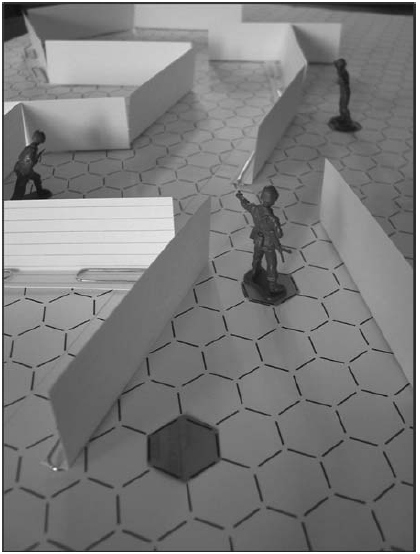
\includegraphics[scale=0.55]{./img/fps-fisical-prototype.png}
 % matrixargseg.png: 296x162 pixel, 100dpi, 7.52x4.11 cm, bb=0 0 213 117
 %\caption{Estágio desenvolvimento de jogos ~\cite{fullerton2008game}}
\caption{Prototipação Física de um \ac{fps} ~\cite{fullerton2008game}}
%  \caption{Estágio desenvolvimento de jogos}
 \label{fig:proto-fps}
\end{figure}

%Uma das etapas do planejamento do designer passa pela concretização da suas ideias através de modelos que consigam certificar de que a concepção é realmente divertida e através de protótipos será possível demonstrá-la para os demais membros da equipe, garantindo que será dada continuidade ao projeto para a produção definitiva ~\cite{prototipgames2007}. Os benefícios do uso de protótipos rápidos é que ele permite testes rápidos de componentes separadamente sem necessariamente implementar o sistema completo como também encoraja usuários a comentar livremente e sugerir modificações (contrário a um produto bem acabado que pode parecer já terminado). Porém, como ponto negativo, temos muitas vezes componentes individuais devem ser re-testados no produto finalizado ~\cite{prototipgames2007}.


%
%
%
%
%\subsection{Protótipo Jogável}
%Game prototypes, while playable, usually include only a rough approximation of the artwork, sound, and features. They are very much like sketches whose purpose is to allow you to focus on a small set of the game’s ~\cite{fullerton2008game}. There are many types of prototypes, including physical prototypes, visual prototypes, video prototypes, software prototypes, etc. 
%
%Prototyping lies at the heart of good game design. Prototyping is the creation of a working model of your idea that allows you to test its feasibility and make improvements to it ~\cite{fullerton2008game}. 
%
%%Buskirk e Moroney [2003] afirmam que o uso da técnica de prototipagem pode ser estendido para outras fases do ciclo de vida do produto além dos testes de usabilidade. Sendo usado na validação dos requisitos junto aos consumidores, na fase de especificação do projeto, desenvolvimento dos manuais do produto, suporte ao marketing, execução de testes funcionais, ajuda no serviço de atendimento aos clientes ~\cite{prototipgames2007}.O público-alvo dessa avaliação inicial inclui publishers, engenheiros de software, artistas, e outros membros da equipe. Como “palavras são fundamentalmente uma maneira terrível de comunicar interatividade” [Waugh 2006], podemos tomar o desenvolvimento de protótipos como meio para ajudar a educar a equipe de como alguns componentes do jogo deveriam se comportar, esclarecendo de forma mais amigável os conceitos abstratos e poder transmitir como o jogo deve funcionar ~\cite{prototipgames2007}.
%If you try to design the entire game at once, you might become confused and overwhelmed. There are so many elements in a typical game that it is diffi cult to know where and how to start. What we recommend is that you isolate the core gameplay mechanisms and build out from there ~\cite{fullerton2008game}.
%
%
%
%\subsection{GAHME Actions Guideline}\label{subsec:game_actions_guide}
%
%Para elaboração deste artefato o \textit{Game Health Designer}, utilizará como irá utilizar as Diretrizes Médicas como base científica de conhecimento e das especificações dos sensores de captura que poderão ser utilizados.
%
%Para elaboração deste artefato o 
%
%Para a sua elaboração o responsável Os artefatos de entrada para elaboração
%
%O responsável pela elaboração do GAHME Actions Design é o que deverá se basear nas Diretrizes Médicas, para fazer uma avaliação dos mPara elaboração do GAHME Actions Design, o autor 
%
%Nesse artefato é levado em consideração o sensor utilizado, o sintoma a ser monitorado e a eficácia do monitoramento sendo comprovada por intermédio de testes efetuados na atividade \textit{Testar Protótipos} da fase de \textit{Prototipação}.
%
%The core gameplay mechanism, or “coremechanic,” can be defi ned as the actions that a player repeats most o en while striving to achieve the game’s overall goal. Games are repetitive by nature. While the meaning and consequences of what a player does can change over the course of game, the core actions tend to remain the same from beginning to end ~\cite{fullerton2008game}.
%
%Creating a physical prototype is a critical step in the design of your original game concept. It will save your team tremendous amounts of time because everyone will have a clear understanding of the game you are making. In addition, a physical prototype will enable you to focus your creative energy on the game mechanics without becoming distracted by the production and programming process ~\cite{fullerton2008game}. 
%
%
%
%\subsection{GAHME Actions Design}
%O objetivo deste artefato é definir quais são os movimentos efetuados pelo jogador dentro do jogo que são passíveis de monitoramento. Para elaboração deste artefato o \textit{GAHME Designer}, irá utilizar as Diretrizes Médicas como base científica de conhecimento e das especificações dos sensores de captura que poderão ser utilizados.
%
%Por promover atividades físicas, ou ações que possam trazer injúria ao jogador, como movimentos de equilíbrio, movimentos repetitivos ou rápidos. O game design do jogo deve ter a preocupação de desenvolver o jogo de acordo com o público-alvo. Isso significa dizer que a faixa etária e limitações físicas e cognitivas em decorrência da idade ou enfermidade devem ser levadas em consideração. Os jogadores devem ter a segurança de usarem o jogo e ter a certeza que o seu uso não acarretará em injúria ~\cite{arntzen2011}.
%
%
%
%
%
%Para elaboração deste artefato o 
%
%Para a sua elaboração o responsável Os artefatos de entrada para elaboração
%
%O responsável pela elaboração do GAHME Actions Design é o que deverá se basear nas Diretrizes Médicas, para fazer uma avaliação dos mPara elaboração do GAHME Actions Design, o autor 
%
%Nesse artefato é levado em consideração o sensor utilizado, o sintoma a ser monitorado e a eficácia do monitoramento sendo comprovada por intermédio de testes efetuados na atividade \textit{Testar Protótipos} da fase de \textit{Prototipação}.
%


